\chapter{\IfLanguageName{dutch}{Stand van zaken}{State of the art}}%
\label{ch:stand-van-zaken}


% Tip: Begin elk hoofdstuk met een paragraaf inleiding die beschrijft hoe
% dit hoofdstuk past binnen het geheel van de bachelorproef. Geef in het
% bijzonder aan wat de link is met het vorige en volgende hoofdstuk.

% Pas na deze inleidende paragraaf komt de eerste sectiehoofding.

%Dit hoofdstuk bevat je literatuurstudie. De inhoud gaat verder op de inleiding, maar zal het onderwerp van de bachelorproef *diepgaand* uitspitten. De bedoeling is dat de lezer na lezing van dit hoofdstuk helemaal op de hoogte is van de huidige stand van zaken (state-of-the-art) in het onderzoeksdomein. Iemand die niet vertrouwd is met het onderwerp, weet nu voldoende om de rest van het verhaal te kunnen volgen, zonder dat die er nog andere informatie moet over opzoeken \autocite{Pollefliet2011}.

%Je verwijst bij elke bewering die je doet, vakterm die je introduceert, enz.\ naar je bronnen. In \LaTeX{} kan dat met het commando \texttt{$\backslash${textcite\{\}}} of \texttt{$\backslash${autocite\{\}}}. Als argument van het commando geef je de ``sleutel'' van een ``record'' in een bibliografische databank in het Bib\LaTeX{}-formaat (een tekstbestand). Als je expliciet naar de auteur verwijst in de zin (narratieve referentie), gebruik je \texttt{$\backslash${}textcite\{\}}. Soms is de auteursnaam niet expliciet een onderdeel van de zin, dan gebruik je \texttt{$\backslash${}autocite\{\}} (referentie tussen haakjes). Dit gebruik je bv.~bij een citaat, of om in het bijschrift van een overgenomen afbeelding, broncode, tabel, enz. te verwijzen naar de bron. In de volgende paragraaf een voorbeeld van elk.

%\textcite{Knuth1998} schreef een van de standaardwerken over sorteer- en zoekalgoritmen. Experten zijn het erover eens dat cloud computing een interessante opportuniteit vormen, zowel voor gebruikers als voor dienstverleners op vlak van informatietechnologie~\autocite{Creeger2009}.

%Let er ook op: het \texttt{cite}-commando voor de punt, dus binnen de zin. Je verwijst meteen naar een bron in de eerste zin die erop gebaseerd is, dus niet pas op het einde van een paragraaf.
\section{\IfLanguageName{dutch}{Basisbegrippen}{Basic concepts}}%
\label{sec:Basisbegrippen}
Om het onderzoeksonderwerp samen met de achterliggende uitdaging te begrijpen, is het belangrijk om de werking van een Public Key Infrastructure (PKI) te begrijpen.
\textcite{Thales2025} definieert een PKI als een set van hardware, software, policies, processen en procedures die noodzakelijk zijn voor het maken, beheren, uitgeven, gebruiken, opslaan en intrekken van digitale certificaten en publieke keys.
PKI's zijn de basis die het gebruik van technologieëen zoals digitale handtekeningen en encryptie mogelijk maakt over een grote populatie van gebruikers.
Zij helpen namelijk met het vaststellen van de identiteit van personen, apparaten en diensten, wat gecontrolleerde toegang tot systemen en bronnen alsook data beveiliging en controle mogelijk maakt. \break

Een groot deel van PKI's zijn Digitale Certificaten en Certificate Authorities (CA's).
Een certificate authority is een bedrijf of organisatie die de identiteit van entiteiten (zoals websites, e-mail adressen, bedrijven, individuen, enz.) valideert en ze vastbindt aan cryptografische sleutels door middel van het uitgeven van electronische documenten gekend als digitale certificaten.
Een certificaat doet zich voor als een getuigschrift dat de identiteit valideert van de entiteit waaraan het is uitgegeven. \autocite{SSLcom} \break

\begin{figure}
  \centering
  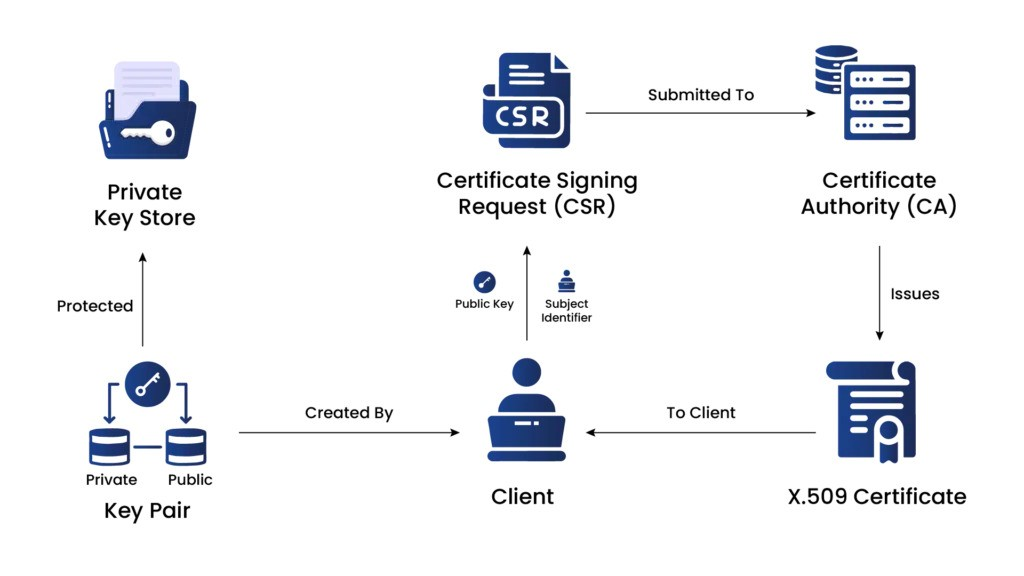
\includegraphics[width=0.8\textwidth]{CertEnr.jpg}
  \caption[Certificate enrollment.]{\label{fig:certenr}Deze afbeelding toont de stappen en componenten in het certificaat uitgave proces.}
\end{figure}

Wanneer een certificaat wordt aangevraagd bij een CA, moet de aanvrager eerst een public en private key genereren. De private key moet onder de controle en eigendom van de aanvrager blijven. In sommige gevallen worden de private keys gegenereerd en veilig bewaart in een Hardware Security Module (HSM). \autocite{SSLcom}
Om de registratie van certificaten te starten, maakt de aanvrager een Certificate Signing Request (CSR) aan. Deze CSR bevat de public key en andere informatie van de aanvrager die in het certificaat zal worden opgenomen, zoals de domeinnaam voor een SSL/TLS certificaat of de aanvrager's e-mail adres voor een S/MIME certificaat.
Daarna wordt de CSR ingedient bij de CA. De CA zal de identiteit van de aanvrager samen met de bijkomende informatie verifiëren. De CA kan verschillende manieren gebruiken om de aanvrager zijn identiteit te verifiëren, zoals e-mail verificatie, domein validatie of manuele validatie van juridische documenten.
Wanneer de CA het verificatie proces heeft voltooid en vaststelt dat de aanvrager legitiem is, zal het digitale certificaat worden uitgegeven. Het certificaat zal de aanvrager zijn public key en bijkomende informatie bevatten, alsook een geldigheidstermijn en de digitale handtekening van de CA.
Het uitgegeven certificaat wordt dan terug gebracht naar de aanvrager, afhankelijk van de CA en het certificaat type zal het certificaat geleverd worden op een verschillende manier zoals via e-mail, een beveiligd portaal of een andere methode.
Na het ontvangen van het certificaat is het aan de aanvrager om het certificaat te installeren op de toepasselijke server of apparaat waar het zal worden gebruikt. Als voorbeeld, een SSL/TLS certificaat wordt geïnstalleerd op een webserver voor een beveiligde connectie naar een website.
Eenmaal het certificaat is geïnstalleerd, kan het gebruikt worden voor protocolen die verantwoordelijk zijn voor beveiligde communicatie. Clients, gebruikers of andere entiteiten die in contact komen met de certificaat eigenaar kunnen de authenticiteit van het certificaat verifiëren aan de hand van de CA zijn digitale handtekening, wat een beveiligde en betrouwbare connectie verzekerd.
Zoals eerder vermeld hebben deze certificaten een geldigheidstermijn (meestal 1 tot 2 jaren). Voor ze vervallen, moet de aanvrager het certificaat vernieuwen via een gelijkaardig proces om het te kunnen blijven gebruiken zonder onderbrekingen. \autocite{EncCon} \break

Het verifiëren van een certificaat om de bepalen of het vertrouwd kan worden is belangrijk voor de veiligheid van de communicatie.
\Textcite{okta} zegt dat tijdens een SSL/TLS handshake, de client het certificaat van de server ontvangt. De client controleert of het certificaat nog niet vervallen is en dat de domeinnaam en IP adres op het certificaat gelijkaardig zijn aan dat van de server. Daarna zal de client kijken of het certificaat correct is ondertekend door een vertrouwde CA.
In de meeste gevallen zal de server certificate niet ondertekend zijn door de root CA die door de client wordt vertrouwd. In plaats van de root CA zal de client 1 of meerdere intermediate CA's vertrouwen zolang als hun ketting van vertrouwen terug leidt naar een root CA die de client vertrouwd.

Voor elke intermediate CA certificate doet de client hetzelfde verificatie proces waarbij de uitgever (issuer) zijn naam overeenkomt met de certificate eigenaar zijn naam van de volgende certificate in de ketting. Ook wordt de digitale signatuur en public key van het certificaat bekeken om te kijken of deze correct is ondertekend.
Dit proces herhaald zichzelf tot de client komt bij een self-signed root CA certificate die de client vertrouwd.
Op dit moment heeft de client dan een cryptografische ketting van vertrouwen gemaakt tot de server en kan de SSL/TLS handshake verder gaan. \break
\begin{figure}
  \centering
  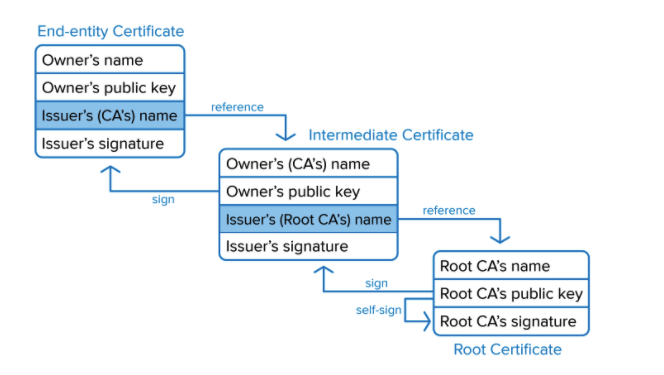
\includegraphics[width=0.8\textwidth]{chainoftrust.png}
  \caption[Chain of trust]{\label{fig:chainoftrust}Deze afbeelding toont de ketting van vertrouwen die de client nakijkt tijdens het verifiëren van een certificaat.}
\end{figure}

Bij dit verificatie proces eindigt de client steeds bij een root CA certificaat die door de client moet worden vertrouwd. Om te bepalen welke root CA's door de client worden vertrouwd bestaan er trust stores.
Een trust store is een collectie van root certificaten die standaard worden vertrouwd door een client en worden beheerd door bedrijven die de client zijn operating system of browser ontwikkelen, zoals Microsoft, Mozilla en Google.
Elke vendor heeft zijn eigen standaarden voor root certificaten maar ze vereisen allemaal dat een uitgevende CA een of meerdere controles ondergaan om hun vertrouwbaarheid, validiteit en conformiteit vast te stellen via de CA/B Forum Baseline Requirements vooraleer ze worden opgenomen in hun trust store. \autocite{Venafi}
Over al de trust stores van deze vendors zijn er heel wat certificaten die niet noodzakelijk zijn. Een studie van \textcite{PerlHenning} toont dat alleen maar 66\% van de certificaten in de trust store van Windows, Linux, MacOS, Firefox, iOS and Android noodzakelijk zijn voor het vertrouwen van websites.
Dit zorgt ervoor dat de overige derde van de root certificaten in de trust stores een potentieel veiligheidsrisico vormen voor de client. \break

Als oplossing hierop kunnen bedrijven het overwegen om deze standaard trust stores af te wijzen. In de plaats daarvan kunnen ze best hun eigen aangepaste, corporate-level trust store maken en gebruik maken van certificate white-listing om te bepalen welke root certificates hierin kunnen opgenomen worden.
Dit helpt bedrijven met het aanvals oppervlak te verkleinen door het limiteren van de hoeveelheid vertrouwde CA's en het markeren van niet-vertrouwde SSL/TLS sessies.
Organisaties kunnen dan deze certificate whitelist en blacklist updaten op een regelmatige basis afhankelijk van benoodigdheden van hun evoluerende business requirements en groeiend CA landschap. \autocite{Venafi} 

Het beheren van deze trust stores kan een uitdaging zijn voor bedrijven, zeker bedrijven met heterogene netwerken (netwerken die clients hebben met verschillende operating systemen en browsers).
\textcite{rfc6024} weerlegt dit door te zeggen dat deze trust anchors (Root CA certificaten) vaak bewaart worden in applicatie-specifieke of OS-specifieke trust stores.
Vaak heeft dan 1 machine een verschillend aantal trust stores die niet gesynchroniseerd zijn met elkaar. \break

De uitdagingen hier zijn dus het vermijden van overbodige vertrouwde root certificaten binnen een netwerk en zijn segmenten afhankelijk van de business requirements en het beheren van deze trust stores over verschillende machines en applicaties. 

\section{\IfLanguageName{dutch}{Verschillende truststores}{Various truststores}}%
\label{sec:Verschillende truststores}

Voor het implementeren van een oplossing voor deze uitdagingen is het van belang om te weten hoe de truststores van de verschillende besturingssystemen en browsers werken en hoe deze kunnen worden beheerd. \break

Windows heeft een truststore die de Trusted Root Certification Authorities store heet.
In de officiële documentatie van Microsoft vermeld \textcite{MStruststore} dat de Trusted Root Certificate Authorities store op een Windows computer via de Microsoft Management Console (MMC) kan worden beheerd door de Certificate Manager snap-in te gebruiken.
De Microsoft Management Console kan worden geopend door het commando \texttt{mmc.exe} uit te voeren in deen Run dialog. In het MCC venster kan men via file -> Add/Remove Snap-in de "Certificates" snap-in toevoegen.
Hierna kan men dan in het MCC venster onder "Certificates (local computer)" -> "Trusted Root Certification Authorities" de lijst van vertrouwde root certificaten bekijken en beheren.
\textcite{MStruststore} vermeld ook dat standaard de Trusted Root Certificate Authorities store geconfigureerd is met een aantal publieke CA's die de vereisten van de Microsoft Root Certificate Program hebben voltooid. \break

Naast de GUI manier van beheren van de truststore, biedt Microsoft ook een manier om het te beheren via de command line aan de hand van het \texttt{certutil} commando.
Certutil.exe is een command-line programma geinstalleerd als onderdeel van de Certitifate Services. Certutil.exe kan gebruikt worden voor het tonen van certificate authority (CA) configuratie informatie, het configureren van Certificate Services en CA componenten te back-uppen en te herstellen.
Dit programma kan ook certificaten, key pairs en certificate chains verifiëren. \autocite{MScertutil}
Om een certificate store te tonen aan de hand van certutil kan het volgende commando worden gebruikt:
\begin{minted}{bash}
  certutil [options] -store [CertificateStoreName [CertId [OutputFile]]]
\end{minted}
Waar CertificateStoreName de naam is van de certificate store, CertId de match token is van het certificaat en OutputFile de naam is van het bestand waarin de overeenkomende certificaten worden opgeslagen. \autocite{MScertutil}

Om een certificaat toe te voegen aan een certificate store kan het volgende commando worden gebruikt:
\begin{minted}{bash}
  certutil [options] -addstore CertificateStoreName InFile
\end{minted}
Waar CertificateStoreName de naam is van de certificate store en InFile de certificate file is die moet worden toegevoegd. \autocite{MScertutil} \break

Linux heeft niet zoals Windows één centrale trust store. In plaats daarvan heeft Linux verschillende trust stores die afhankelijk zijn van de applicatie of fr distributie van Linux.

Binnen Ubuntu Server moet een certificaat in PEM formaat staan vooraleer het kan worden toegevoegd aan de trust store.
Om een PEM-geformatteerd root CA certificaat met als voorbeeld naam "local-ca.crt" te installeren in de trust store van Ubuntu Server kan het volgende commando worden gebruikt:
\begin{minted}{bash}
  sudo apt-get install -y ca-certificates
  sudo cp local-ca.crt /usr/local/share/ca-certificates
  sudo update-ca-certificates
\end{minted}

Het is hierbij belangrijk dat het certificaat bestand de extensie .crt heeft anders zal het niet worden verwerkt.

De trust store (die gegenereerd wordt door update-ca-certificates) is te vinden op de volgende locaties:
\begin{itemize}
  \item Als een file (PEM bundel) in /etc/ssl/certs/ca-certificates.crt
  \item Als een OpenSSL-compatibele certificaat directory in /etc/ssl/certs/ca-certificates.pem
\end{itemize} \autocite{UbunTruststore}
\break

Red Hat Enterprise Linux (RHEL) heeft een andere manier van het beheren van de trust store. RHEL biedt de Shared System Certificates aan.
De Shared System Certificates storage laat NSS, GnuTLS, OpenSSL en Java toe om een standaard bron te delen voor het ophalen van systeem certificate anchors en black list informatie.
Standaard bevat de truststore de Mozilla CA list, die positieve en negatieve trust informatie bevat. Het systeem laat toe om de Mozilla CA lijst aan te passen of om een andere CA lijst te gebruiken. \autocite{RHELtruststore} \break

In Red Hat Enterprise Linux 7 is de systeem-brede truststore te vinden in de directories /etc/pki/ca-trust/ en /usr/share/pki/ca-trust-source/ . De trust settings in /usr/share/pki/ca-trust-source/ worden behandeld met een lagere prioriteit dan de settings in /etc/pki/ca-trust/ .
Certificaat bestanden worden anders behandeld afhankelijk van de subdirectory waarin ze worden geplaatst:
\begin{itemize}
  \item /usr/share/pki/ca-trust-source/anchors/ of /etc/pki/ca-trust/source/anchors/ : voor trust anchors.
  \item /usr/share/pki/ca-trust-source/blacklist/ of /etc/pki/ca-trust/source/blacklist/ : voor niet vertrouwde certificaten.
  \item /usr/share/pki/ca-trust-source/ of /etc/pki/ca-trust/source/ : voor certificaten in de extended BEGIN TRUSTED bestandsformaat.
\end{itemize} \autocite{RHELtruststore}

Om een certificaat in de simpele PEM of DER bestandsformaten aan de lijst van vertrouwde CA's op het systeem toe te voegen, kan je simpelweg het certificaat bestand kopiëren naar de /usr/share/pki/ca-trust-source/anchors/ of /etc/pki/ca-trust/source/anchors/ directory. Om de systeem-brede truststore te updaten ka je het update-ca-trust commando gebruiken zoals volgt:
\begin{minted}{bash}
  cp ~/certificate-trust-examples/Cert-trust-test-ca.pem /usr/share/pki/ca-trust-source/anchors/
  update-ca-trust
\end{minted} 

Om de trust anchors op te lijsten, toe te voegen, veranderen of verwijderen kan het 'trust' commando gebruikt worden.
Voor het oplijsten van de trust anchors wordt 'trust list' gebruikt.
Een trust anchor opslaan in de trust store kan met het 'trust anchor' sub-commando en het specifiëren van het pad (vb.: 'path.to') naar het certificaat bestand, zoals volgt:
\begin{minted}{bash}
  trust anchor path.to/certificate.crt
\end{minted} 
Om een trust anchor te verwijderen kan een pad naar het certificaat of ID van het certificaat gebruikt worden:
\begin{minted}{bash}
  trust anchor --remove path.to/certificate.crt
  trust anchor --remove "pkcs11:id=%AA%BB%CC%DD%EE;type=cert"
\end{minted} 
\autocite{RHELtruststore} \break

Applicaties kunnen ook hun eigen trust store hebben. Een voorbeeld hiervan is Mozilla Firefox. Firefox maakt gebruik van de NSS (Network Security Services) library voor het beheren van de trust store.
De Network Security Services (NSS) library is een set van libraries ontwikkeld om cross-platform ontwikkeling van veilige client en server applicaties te ondersteunen. De libraries ondersteunen SSL v3, TLS, PKCS #5, PKCS #7, PKCS #11, PKCS #12, S/MIME, X.509 v3 certificaten en andere security standaarden. \autocite{FirefoxNNS}
Firefox geeft bij initiatie een string met pad naar de directory waar NSS de security en configuratie data mag opslaan. NSS slaat 3 bestanden op in die directory:
\begin{itemize}
  \item cert8.db: slaat publiek toegankelijke objecten op (Certificaten, CRL's, S/MIME records).
  \item key3.db: slaat private keys op.
  \item secmod.db: slaat de PKCS#11 module configuratie op.
\end{itemize}
Als in deze directory grote security objecten zitten (zoals grote CRL's), zal NSS deze opslaan in bestanden in subdirectories genaamd 'cert8.dir'.
In het geval dat cert8.db en/of key3.db niet bestaan, zal NSS de data lezen van oudere versies vand eze databases (bv.: cert7.db, cert6.db,...) en zal deze data gebruiken om een nieuwe cert8.db en key3.db te maken. \autocite{MozillaWiki}

Ook beweert \textcite{MozillaCA} dat standaard Firefox op Windows, MacOS en Android zal zoeken en gebruik maken van de third-party CA's die zijn opgenomen in de operating system zijn trust store.
Firefox kan geconfigureerd worden om automatisch te zoeken naar CA's die in de Windows certificate store zijn toegevoegd door een gebruiker of administrator. Dit kan gedaan worden door de \texttt{security.enterprise_roots.enabled} optie in te stellen op 'true' in de config van Firefox.
Firefox zal dan de HKLM/SOFTWARE/Microsoft/SystemCertificates (Het pad dat overeenstemt met de API flag CERT\_SYSTEM\_STORE\_LOCAL\_MACHINE) registry directory inspecteren voor CA's die vertrouwd worden om certiifcaten uit te geven voor TLS web server authenticatie. \autocite{MozillaCA}
Ook wordt er gekeken naar de volgende andere locaties:
\begin{itemize}
  \item HKLM/SOFTWARE/Policies/Microsoft/SystemCertificates/Root/Certificates (pad in API flag CERT\_SYSTEM\_STORE\_LOCAL\_MACHINE\_GROUP\_POLICY)
  \item HKLM/SOFTWARE/Microsoft/EnterpriseCertificates/Root/Certificates (pad in API flag CERT\_SYSTEM\_STORE\_LOCAL\_MACHINE\_ENTERPRISE)
\end{itemize} \autocite{MozillaCA}

\textcite{MozillaCA} voorziet ook dat enterprise policies kunnen gebruikt worden voor het toevoegen van CA certificaten in Firefox.
De 'ImportEnterpriseRoots' key op 'true' zetten, zorgt ervoor dat Firefox root certificaten zal vertrouwen.
De 'Install' key zoekt standaard naar certificaten in de onderstaande locaties. Er kan ook een specifiek pad worden opgegeven. Als Firefox daar geen certificaten vindt zal het de standaard directories bekijken:
\begin{itemize}
  \item Windows
  \begin{itemize}
    \item \%USERPROFILE\%\symbol{92}AppData\symbol{92}Local\symbol{92}Mozilla\symbol{92}Certificates 
    \item \%USERPROFILE\%\symbol{92}AppData\symbol{92}Roaming\symbol{92}Mozilla\symbol{92}Certificates
  \end{itemize}

  \item macOS
  \begin{itemize}
    \item /Library/Application Support/Mozilla/Certificates 
    \item ~/Library/Application Support/Mozilla/Certificates 
  \end{itemize}

  \item Linux 
  \begin{itemize}
    \item /usr/lib/mozilla/certificates 
    \item /usr/lib64/mozilla/certificates 
  \end{itemize}
\end{itemize} \autocite{MozillaCA} \break

\section{\IfLanguageName{dutch}{Bestaande tools}{Existing tools}}%
\label{sec:Bestaande tools}

Er bestaan verschillende gratis tools die kunnen helpen met het beheren van truststores over verschillende machines en applicaties.
Deze tools zijn niet ontwikkeld specifiek voor het beheren van truststores maar bieden functionaliteiten aan voor het beheren van end-points hun configuratie.
Voor Windows bestaat Microsoft System Center Configuration Manager (SCCM).

\textcite{ConfigMan} zegt dat Configuration Manager deel uitmaakt van de Microsoft Intune familie van producten. De Microsoft Intune familie van producten is een geïntegreerde oplossing voor het beheren van al jouw apparaten.
Configuration Manager vebreed en werkt samen met vele Microsoft technologieëen en oplossing zoals onder andere Certificate Services.

Een meer algemene oplossing die werkt voor beide Windows en Linux is Ansible.
Ansible is een open-source IT automation engine die provisioning, configuratie management, applicatie deployment, orkestratie en vele andere IT taken automatiseert.
Ansible kan gratis worden gebruikt en het project profiteert van de ervanging en intelligentie van zijn duizende gebruikers. \autocite{Ansible}

Ansible zijn grootste sterkte is eenvoud. Het heeft ook een sterke focus op beveiliging en betrouwbaarheid, met zo weinig mogelijk bewegende delen. Het gebruikt OpenSSH voor transport (met andere transport en pull modes beschikbaar als alternatieven), en gebruikt leesbare taal die ontworpen is om snel aan de start te kunnen gaan zonder enige training.
Red Hat Ansible Automation Platform is een abbonement gebaseerde oplossing die bouwt op de basis van Ansible met een aantal ondernemingsgerichte functionaliteiten.
Beide community Ansible en Ansible Automation Platform zijn gebouwt op het concept van een control node en een managed node. Ansible wordt gebruikt op de control node waar bijvoorbeeld een gebruiker een ansible-playbook command uitvoert. Managed nodes zijn de apparaten die worden geautomatiseerd zoals bijvoorbeeld een Windows server.
Voor Linux en Windows te automatiseren, connecteert Ansible met de managed nodes en verstuurt het kleine programma's genaamd Andisble modules uit. Deze programma's zijn geschreven als bronmodellen van de gewenste staat van het systeem. Ansible voert dan deze modules uit (standaard over SSH), en verwijdert ze na ze voltooien.
Deze modules zijn ontworpen om idempotent te zijn waar mogelijk, zodanig ze alleen een aanpassing uitvoeren op een systeem als dat nodig is. \autocite{AnisbleHow} \break

Een andere tool die mogelijks kan helpen is Open Source Puppet.
Puppet is een open source configuratie management tool geproduceert door Puppet Labs. Er kunnen systeem configuraties gedefinieerd worden aan de hand van Puppet's declaratieve taal en deze configuraties kunnen dan opgeslagen worden in bestanden genaamd Puppet Manifests.
Puppet kan standalone op een systeem draaien of in een agent/master configuratie. Met standalone Puppet draaien systemen het programma lokaal om hun eigen configuraties aan te passen. Met agent/master Puppet beheert een centrale Puppet master server of servers meerdere systemen die de Puppet agent draaien.
Bij beide implementaties worden Puppet manifests gebruikt om systeem configuraties naar de verwachte staat te brengen. Daarnaast bestaat er ook nog een commerciële versie van Puppet genaamd Puppet Enterprise. \autocite{Puppet} \break

Naast Ansible en Puppet bestaan er ook nog andere tools zoals Saltstack en Chef.
Gebouwt op Python, is Salt een event-driven automatiseringstool en framework dat is ontworpen om complexe IT systemen te deployeren, configureren en beheren. Salt kan gebruikt worden voor veel voorkomende administratie taken te automatiseren en te verzekeren dat alle componenten van je infrastructuur operationeel zijn in de verwachte staat.
Salt heeft vele mogelijke gebruiksdoeleinden, zoals configuratie beheer, wat als volgt inhoud:
\begin{itemize}
  \item Het beheren van het deployeren van besturingssystemen en hun configuratie.
  \item Het installeren en configureren van software applicaties en diensten.
  \item Het beheren servers, virtuele machines, containers, databases, web servers, netwerk apparaten en meer.
  \item Verzekeren dat de configuratie consistent is en het vermijden van drift.
\end{itemize}

Salt maakt het mogelijk om applicaties te implementeren en beheren die gebruik maken van elke technologiestack die op bijna elk besturingssysteem draait, inclusief verschilllende soorten netwerkapparaten zoals switches en routers van verschillende leveranciers.
Daarnaast kan het ook gebruikt worden voor het automatiseren en orkestreren van routine IT processen zoals veel voorkomende noodzakelijke taken voor geplande server downtime of het upgraden van besturingssystemen en applicaties. 
Ook kan Salt gebruikt worden om een zelfbewuste, zelf herstellende systemen te maken die automatisch kunnen reageren op uitvallingen, veel voorkomende administratie problemen of andere belangrijke gebeurtenissen. \autocite{Saltstack} \break

\textcite{Chef} noemt Chef een automation company. Vandaag biedt Chef automatiseringsoplossingen voor beide infrasctructuur en applicaties van ontwikkeling tot productie.
Chef Infra automatiseert hoe infrastructuur is geconfigureerd, gedeployed en beheerd doorheen het netwerk, ongeacht de grootte.

Chef Workstation maakt het mogelijk om 'cookbooks' te schrijven en je infrastructuur te beheren. Chef Workstation hoort te draaien op de machine die je dagelijks gebruikt, ongeacht of deze Windows, Linux of MacOS draait.
Eenmaal het ontwikkelen van je code gedaan is op je workstation, dan kan je deze code uploaden naar de CHef Infra Server. De Chef Infra Server is een centrale opslagplaats voor je configuratie data. Het slaat cookbooks, policies en metadata van elk systeem op. Het communiceren met de Chef Infra Server vanaf een workstation kan via het 'knife' commando.
Chef Infra Clients contacteren deze Chef Infra Server periodiek om de laatste cookbooks op te halen. Als de huidige staat van de node niet overeenstemt met wat de cookbook beschrijft, zal de Chef Infra Client de cookbook instrucites uitvoeren. \autocite{Chef} \break

\section{\IfLanguageName{dutch}{Infrastructuur studie}{Infrastructure study}}%
\label{sec:Infrastructuur studie}

Voor een realistisch beeld te scheppen van een bedrijfsomgeving, zal er gekeken worden naar resultaten van meerdere vragenlijsten en enquêtes die het marktaandeel van verschillende technologieëen onderzoeken. \break

\textcite{NetcraftSurvey} publiceert maandelijks een web server survey waarin ze de marktaandelen van web servers onderzoeken, uit de resultaten van de survey van januari 2025 blijkt Nginx het grootste marktaandeel te hebben binnen alle onderzochte sites met 19,60\% alsook alle onderzochte actieve sites met 18,89\%.
Naast Nginx heeft Apache het tweede grootste marktaandeel met 16,96\% van alle onderzochte sites en 17,24\% van alle actieve sites. \break

Binnen de Stack Overflow developer survey van 2024 kan er ook gekeken worden naar veel gebruikte technologieëen binnen de professionele wereld.
In de resultaten kan er gekeken worden naar welke van de eerder vermelde tools het meest gebruikt worden in de professionele wereld. \autocite{StackOverflowSurvey} rapporteert onder overige tools dat Ansible gebruikt wordt door 8,1\% van de ondervraagde professionele developers, Pupper door 1,1\% en Chef door 0,7\%. \break

Binnen de resultaten van de Stack Overflow survey kan er ook gekeken worden naar de meest gebruikte databases. Uit deze resultaten blijkt dat PostgreSQL de meest gebruikte database is met 51,9\% van de ondervraagde professionele developers die het gebruiken. MySQL is de tweede meest gebruikte database met 39,4\% van de ondervraagde professionele developers die het gebruiken. \autocite{StackOverflowSurvey} \break

Het bepalen welke DNS server technologie het meest gebruikt wordt binnen bedrijven is moeilijk omdat dit geen publiek beschikbare data is. Hier zal BIND gekozen worden, volgens \textcite{Bind9} is BIND 9 de eerste, oudste en meest gebruikte oplossing waarmee netwerk engineers al meer bekend zijn dan met andere systemen. \break

\textcite{SecSpMail} publiceert ook rapporten op verschillende technologieëen. Een van deze rapporten bestudeert alle zichtbare mailservers op het internet en kijkt naar welke onderliggende software ze gebruiken. Uit de resultaten van Maart 2025 blijkt dat Exim de meest gebruikte mailserversoftware is met 55,05\% en Postfix de tweede meest gebruikte met 38,52\%. \break

Deze informatie zal gebruikt worden voor het bepalen van de gebruikte technologieëen binnen de proof-of-concept virtuele omgeving.
%\begin{figure}
%  \centering
%  \includegraphics[width=0.8\textwidth]{grail.jpg}
%  \caption[Voorbeeld figuur.]{\label{fig:grail}Voorbeeld van invoegen van een figuur. Zorg altijd voor een uitgebreid bijschrift dat de figuur volledig beschrijft zonder in de tekst te moeten gaan zoeken. Vergeet ook je bronvermelding niet!}
%\end{figure}

%\begin{listing}
%  \begin{minted}{python}
%    import pandas as pd
%    import seaborn as sns
%
%    penguins = sns.load_dataset('penguins')
%    sns.relplot(data=penguins, x="flipper_length_mm", y="bill_length_mm", hue="species")
%  \end{minted}
%  \caption[Voorbeeld codefragment]{Voorbeeld van het invoegen van een codefragment.}
%\end{listing}

%\lipsum[7-20]

%\begin{table}
%  \centering
%  \begin{tabular}{lcr}
%    \toprule
%    \textbf{Kolom 1} & \textbf{Kolom 2} & \textbf{Kolom 3} \\
%    $\alpha$         & $\beta$          & $\gamma$         \\
%    \midrule
%    A                & 10.230           & a                \\
%    B                & 45.678           & b                \\
%    C                & 99.987           & c                \\
%    \bottomrule
%  \end{tabular}
%  \caption[Voorbeeld tabel]{\label{tab:example}Voorbeeld van een tabel.}
%\end{table}

